% Options for packages loaded elsewhere
% Options for packages loaded elsewhere
\PassOptionsToPackage{unicode}{hyperref}
\PassOptionsToPackage{hyphens}{url}
\PassOptionsToPackage{dvipsnames,svgnames,x11names}{xcolor}
%
\documentclass[
  letterpaper,
  DIV=11,
  numbers=noendperiod]{scrartcl}
\usepackage{xcolor}
\usepackage{amsmath,amssymb}
\setcounter{secnumdepth}{5}
\usepackage{iftex}
\ifPDFTeX
  \usepackage[T1]{fontenc}
  \usepackage[utf8]{inputenc}
  \usepackage{textcomp} % provide euro and other symbols
\else % if luatex or xetex
  \usepackage{unicode-math} % this also loads fontspec
  \defaultfontfeatures{Scale=MatchLowercase}
  \defaultfontfeatures[\rmfamily]{Ligatures=TeX,Scale=1}
\fi
\usepackage{lmodern}
\ifPDFTeX\else
  % xetex/luatex font selection
\fi
% Use upquote if available, for straight quotes in verbatim environments
\IfFileExists{upquote.sty}{\usepackage{upquote}}{}
\IfFileExists{microtype.sty}{% use microtype if available
  \usepackage[]{microtype}
  \UseMicrotypeSet[protrusion]{basicmath} % disable protrusion for tt fonts
}{}
\makeatletter
\@ifundefined{KOMAClassName}{% if non-KOMA class
  \IfFileExists{parskip.sty}{%
    \usepackage{parskip}
  }{% else
    \setlength{\parindent}{0pt}
    \setlength{\parskip}{6pt plus 2pt minus 1pt}}
}{% if KOMA class
  \KOMAoptions{parskip=half}}
\makeatother
% Make \paragraph and \subparagraph free-standing
\makeatletter
\ifx\paragraph\undefined\else
  \let\oldparagraph\paragraph
  \renewcommand{\paragraph}{
    \@ifstar
      \xxxParagraphStar
      \xxxParagraphNoStar
  }
  \newcommand{\xxxParagraphStar}[1]{\oldparagraph*{#1}\mbox{}}
  \newcommand{\xxxParagraphNoStar}[1]{\oldparagraph{#1}\mbox{}}
\fi
\ifx\subparagraph\undefined\else
  \let\oldsubparagraph\subparagraph
  \renewcommand{\subparagraph}{
    \@ifstar
      \xxxSubParagraphStar
      \xxxSubParagraphNoStar
  }
  \newcommand{\xxxSubParagraphStar}[1]{\oldsubparagraph*{#1}\mbox{}}
  \newcommand{\xxxSubParagraphNoStar}[1]{\oldsubparagraph{#1}\mbox{}}
\fi
\makeatother

\usepackage{color}
\usepackage{fancyvrb}
\newcommand{\VerbBar}{|}
\newcommand{\VERB}{\Verb[commandchars=\\\{\}]}
\DefineVerbatimEnvironment{Highlighting}{Verbatim}{commandchars=\\\{\}}
% Add ',fontsize=\small' for more characters per line
\usepackage{framed}
\definecolor{shadecolor}{RGB}{241,243,245}
\newenvironment{Shaded}{\begin{snugshade}}{\end{snugshade}}
\newcommand{\AlertTok}[1]{\textcolor[rgb]{0.68,0.00,0.00}{#1}}
\newcommand{\AnnotationTok}[1]{\textcolor[rgb]{0.37,0.37,0.37}{#1}}
\newcommand{\AttributeTok}[1]{\textcolor[rgb]{0.40,0.45,0.13}{#1}}
\newcommand{\BaseNTok}[1]{\textcolor[rgb]{0.68,0.00,0.00}{#1}}
\newcommand{\BuiltInTok}[1]{\textcolor[rgb]{0.00,0.23,0.31}{#1}}
\newcommand{\CharTok}[1]{\textcolor[rgb]{0.13,0.47,0.30}{#1}}
\newcommand{\CommentTok}[1]{\textcolor[rgb]{0.37,0.37,0.37}{#1}}
\newcommand{\CommentVarTok}[1]{\textcolor[rgb]{0.37,0.37,0.37}{\textit{#1}}}
\newcommand{\ConstantTok}[1]{\textcolor[rgb]{0.56,0.35,0.01}{#1}}
\newcommand{\ControlFlowTok}[1]{\textcolor[rgb]{0.00,0.23,0.31}{\textbf{#1}}}
\newcommand{\DataTypeTok}[1]{\textcolor[rgb]{0.68,0.00,0.00}{#1}}
\newcommand{\DecValTok}[1]{\textcolor[rgb]{0.68,0.00,0.00}{#1}}
\newcommand{\DocumentationTok}[1]{\textcolor[rgb]{0.37,0.37,0.37}{\textit{#1}}}
\newcommand{\ErrorTok}[1]{\textcolor[rgb]{0.68,0.00,0.00}{#1}}
\newcommand{\ExtensionTok}[1]{\textcolor[rgb]{0.00,0.23,0.31}{#1}}
\newcommand{\FloatTok}[1]{\textcolor[rgb]{0.68,0.00,0.00}{#1}}
\newcommand{\FunctionTok}[1]{\textcolor[rgb]{0.28,0.35,0.67}{#1}}
\newcommand{\ImportTok}[1]{\textcolor[rgb]{0.00,0.46,0.62}{#1}}
\newcommand{\InformationTok}[1]{\textcolor[rgb]{0.37,0.37,0.37}{#1}}
\newcommand{\KeywordTok}[1]{\textcolor[rgb]{0.00,0.23,0.31}{\textbf{#1}}}
\newcommand{\NormalTok}[1]{\textcolor[rgb]{0.00,0.23,0.31}{#1}}
\newcommand{\OperatorTok}[1]{\textcolor[rgb]{0.37,0.37,0.37}{#1}}
\newcommand{\OtherTok}[1]{\textcolor[rgb]{0.00,0.23,0.31}{#1}}
\newcommand{\PreprocessorTok}[1]{\textcolor[rgb]{0.68,0.00,0.00}{#1}}
\newcommand{\RegionMarkerTok}[1]{\textcolor[rgb]{0.00,0.23,0.31}{#1}}
\newcommand{\SpecialCharTok}[1]{\textcolor[rgb]{0.37,0.37,0.37}{#1}}
\newcommand{\SpecialStringTok}[1]{\textcolor[rgb]{0.13,0.47,0.30}{#1}}
\newcommand{\StringTok}[1]{\textcolor[rgb]{0.13,0.47,0.30}{#1}}
\newcommand{\VariableTok}[1]{\textcolor[rgb]{0.07,0.07,0.07}{#1}}
\newcommand{\VerbatimStringTok}[1]{\textcolor[rgb]{0.13,0.47,0.30}{#1}}
\newcommand{\WarningTok}[1]{\textcolor[rgb]{0.37,0.37,0.37}{\textit{#1}}}

\usepackage{longtable,booktabs,array}
\usepackage{calc} % for calculating minipage widths
% Correct order of tables after \paragraph or \subparagraph
\usepackage{etoolbox}
\makeatletter
\patchcmd\longtable{\par}{\if@noskipsec\mbox{}\fi\par}{}{}
\makeatother
% Allow footnotes in longtable head/foot
\IfFileExists{footnotehyper.sty}{\usepackage{footnotehyper}}{\usepackage{footnote}}
\makesavenoteenv{longtable}
\usepackage{graphicx}
\makeatletter
\newsavebox\pandoc@box
\newcommand*\pandocbounded[1]{% scales image to fit in text height/width
  \sbox\pandoc@box{#1}%
  \Gscale@div\@tempa{\textheight}{\dimexpr\ht\pandoc@box+\dp\pandoc@box\relax}%
  \Gscale@div\@tempb{\linewidth}{\wd\pandoc@box}%
  \ifdim\@tempb\p@<\@tempa\p@\let\@tempa\@tempb\fi% select the smaller of both
  \ifdim\@tempa\p@<\p@\scalebox{\@tempa}{\usebox\pandoc@box}%
  \else\usebox{\pandoc@box}%
  \fi%
}
% Set default figure placement to htbp
\def\fps@figure{htbp}
\makeatother


% definitions for citeproc citations
\NewDocumentCommand\citeproctext{}{}
\NewDocumentCommand\citeproc{mm}{%
  \begingroup\def\citeproctext{#2}\cite{#1}\endgroup}
\makeatletter
 % allow citations to break across lines
 \let\@cite@ofmt\@firstofone
 % avoid brackets around text for \cite:
 \def\@biblabel#1{}
 \def\@cite#1#2{{#1\if@tempswa , #2\fi}}
\makeatother
\newlength{\cslhangindent}
\setlength{\cslhangindent}{1.5em}
\newlength{\csllabelwidth}
\setlength{\csllabelwidth}{3em}
\newenvironment{CSLReferences}[2] % #1 hanging-indent, #2 entry-spacing
 {\begin{list}{}{%
  \setlength{\itemindent}{0pt}
  \setlength{\leftmargin}{0pt}
  \setlength{\parsep}{0pt}
  % turn on hanging indent if param 1 is 1
  \ifodd #1
   \setlength{\leftmargin}{\cslhangindent}
   \setlength{\itemindent}{-1\cslhangindent}
  \fi
  % set entry spacing
  \setlength{\itemsep}{#2\baselineskip}}}
 {\end{list}}
\usepackage{calc}
\newcommand{\CSLBlock}[1]{\hfill\break\parbox[t]{\linewidth}{\strut\ignorespaces#1\strut}}
\newcommand{\CSLLeftMargin}[1]{\parbox[t]{\csllabelwidth}{\strut#1\strut}}
\newcommand{\CSLRightInline}[1]{\parbox[t]{\linewidth - \csllabelwidth}{\strut#1\strut}}
\newcommand{\CSLIndent}[1]{\hspace{\cslhangindent}#1}



\setlength{\emergencystretch}{3em} % prevent overfull lines

\providecommand{\tightlist}{%
  \setlength{\itemsep}{0pt}\setlength{\parskip}{0pt}}



 


\usepackage{booktabs}
\usepackage{caption}
\usepackage{longtable}
\usepackage{colortbl}
\usepackage{array}
\usepackage{anyfontsize}
\usepackage{multirow}
\KOMAoption{captions}{tableheading}
\makeatletter
\@ifpackageloaded{caption}{}{\usepackage{caption}}
\AtBeginDocument{%
\ifdefined\contentsname
  \renewcommand*\contentsname{Table of contents}
\else
  \newcommand\contentsname{Table of contents}
\fi
\ifdefined\listfigurename
  \renewcommand*\listfigurename{List of Figures}
\else
  \newcommand\listfigurename{List of Figures}
\fi
\ifdefined\listtablename
  \renewcommand*\listtablename{List of Tables}
\else
  \newcommand\listtablename{List of Tables}
\fi
\ifdefined\figurename
  \renewcommand*\figurename{Figure}
\else
  \newcommand\figurename{Figure}
\fi
\ifdefined\tablename
  \renewcommand*\tablename{Table}
\else
  \newcommand\tablename{Table}
\fi
}
\@ifpackageloaded{float}{}{\usepackage{float}}
\floatstyle{ruled}
\@ifundefined{c@chapter}{\newfloat{codelisting}{h}{lop}}{\newfloat{codelisting}{h}{lop}[chapter]}
\floatname{codelisting}{Listing}
\newcommand*\listoflistings{\listof{codelisting}{List of Listings}}
\makeatother
\makeatletter
\makeatother
\makeatletter
\@ifpackageloaded{caption}{}{\usepackage{caption}}
\@ifpackageloaded{subcaption}{}{\usepackage{subcaption}}
\makeatother
\usepackage{bookmark}
\IfFileExists{xurl.sty}{\usepackage{xurl}}{} % add URL line breaks if available
\urlstyle{same}
\hypersetup{
  pdftitle={Impact of Subgroup Misclassification on Detecting Heterogeneous Treatment Effects in Staphylococcus aureus Bacteremia: A Simulation Study},
  pdfauthor={Fergus Hamilton},
  colorlinks=true,
  linkcolor={blue},
  filecolor={Maroon},
  citecolor={Blue},
  urlcolor={Blue},
  pdfcreator={LaTeX via pandoc}}


\title{Impact of Subgroup Misclassification on Detecting Heterogeneous
Treatment Effects in \emph{Staphylococcus aureus} Bacteremia: A
Simulation Study}
\author{Fergus Hamilton}
\date{2025-07-14}
\begin{document}
\maketitle

\renewcommand*\contentsname{Table of contents}
{
\hypersetup{linkcolor=}
\setcounter{tocdepth}{3}
\tableofcontents
}

\section{Abstract}\label{abstract}

\textbf{Background:} \emph{Staphylococcus aureus} bacteremia (SAB)
exhibits significant clinical heterogeneity. Recently identified
subphenotypes show potential for heterogeneous treatment effects (HTE),
but the impact of inevitable patient misclassification on detecting HTE
is unclear.

\textbf{Methods:} We conducted a simulation study following the ADEMP
framework (Aims, Data-generating mechanisms, Estimands, Methods,
Performance measures). We simulated clinical trial data based on
parameters from the ARREST trial (adjunctive rifampicin vs.~placebo for
SAB), incorporating five subphenotypes with differential treatment
effects on 84-day mortality (Odds Ratios {[}ORs{]} from 0.3 to 18.8). We
assessed: (1) statistical power for post-hoc subgroup analysis versus
total trial size assuming perfect classification; (2) the impact of
varying classification accuracy (50\%-100\%) on power, bias, MSE, and
wrong-direction estimate rate in post-hoc analyses (fixed N=10,000); and
(3) the Number Needed to Screen (NNS) and Number Needed to Randomize
(NNR) to achieve 80\% power in enrichment trials targeting specific
subgroups, considering test accuracy. Simulations were repeated using
more moderate (`realistic') ORs.

\textbf{Results:} Aim 1 showed substantial total trial sizes
(\textgreater20,000) are needed for adequate power (80\%) in post-hoc
analyses of some subgroups (B, C, E) even with perfect classification,
largely driven by low baseline event rates or moderate effect sizes
combined with multiple testing correction. Aim 2 demonstrated that
decreasing classification accuracy markedly reduced power and increased
bias (towards the null) and the risk of estimating effects in the wrong
direction in post-hoc analyses. Aim 3 showed that enrichment designs
require large NNS, increasing dramatically as test accuracy decreases;
for subgroup B (OR=18.8), NNS exceeded 50,000 even with 95\% accuracy.
Results were less extreme but directionally similar for realistic ORs.

\textbf{Conclusions:} Detecting HTE in SAB is challenging. Post-hoc
analyses require very large trials and high classification accuracy.
Enrichment strategies can reduce NNR but face substantial screening
burdens (NNS) heavily influenced by test accuracy and subgroup
prevalence. Robust classification methods are crucial for advancing
stratified medicine approaches in SAB.

\section{Introduction}\label{introduction}

\emph{Staphylococcus aureus} bacteremia (SAB) is a common and serious
infection associated with significant morbidity and mortality (1).
Globally, \emph{S. aureus} is a leading cause of death due to bacterial
pathogens and bacteremia (2). A defining feature of SAB is its clinical
heterogeneity, encompassing variations in patient characteristics (e.g.,
age, comorbidities), pathogen factors (e.g., methicillin resistance),
source of infection, and disease severity (1). Despite this
heterogeneity, clinical trials in SAB often treat it as a single entity,
potentially obscuring differential treatment effects within patient
subgroups {[}(3); Holland2022{]}. Strategy trials investigating
adjunctive or alternative therapies have frequently failed to show
overall benefit compared to standard care {[}(3); Paulsen2024{]}.

Recent efforts have focused on identifying clinically relevant
subphenotypes within SAB to enable better patient stratification for
research and potentially personalized treatment (4). Swets, Russell, et
al.~recently used latent class analysis on data from observational and
trial cohorts (Edinburgh, ARREST, SAFO) to identify five distinct and
reproducible clinical subphenotypes (A-E) based on routinely collected
clinical data (5). Crucially, a secondary analysis of the ARREST trial
(Adjunctive Rifampicin for \emph{S. aureus} Bacteraemia) suggested
potential heterogeneous treatment effects (HTE) of adjunctive rifampicin
across these subphenotypes regarding 84-day mortality. Notably,
rifampicin appeared potentially harmful in subphenotype B (Nosocomial IV
catheter-associated SAB; OR 18.8) and potentially beneficial in
subphenotype E (SAB associated with injecting drug use; OR 0.3) (5).

The possibility of such HTE raises critical questions for future
clinical trial design and the implementation of stratified medicine
approaches. If treatment effects truly differ between subgroups,
accurately identifying these subgroups becomes paramount. However, any
diagnostic test or classification algorithm used to assign patients to
subphenotypes will inevitably have imperfect accuracy (6).
Misclassifying patients can lead to biased estimates of
subgroup-specific effects, reduced statistical power to detect true HTE,
and potentially misleading conclusions about which patients benefit or
are harmed by a treatment {[}(7); Sussman2017{]}. Understanding the
quantitative impact of misclassification is essential for interpreting
subgroup analyses and designing efficient trials, including potential
enrichment strategies {[}(8); Simon2004{]}.

This simulation study aims to quantify the impact of subgroup
misclassification on detecting HTE in SAB, using the subphenotypes and
treatment effects derived from the Swets et al.~analysis of the ARREST
trial as a motivating example. Specifically, we address three aims: 1.
Estimate the total sample sizes required in a standard randomized
controlled trial (RCT) to achieve adequate statistical power (80\%) for
post-hoc analyses of subgroup-specific treatment effects (based on
ARREST trial ORs) in post-hoc analyses, assuming perfect patient
classification. 2. Quantify the impact of varying levels of
classification accuracy (0.5 to 1.0) on statistical power, bias, MSE,
and the wrong-direction rate for estimating subgroup-specific and
overall treatment effects in post-hoc analyses of a standard RCT with a
fixed total sample size (\texttt{n}=10,000). 3. Estimate the Number
Needed to Screen (NNS) and the average Number Needed to Randomize (NNR)
within the enriched cohort required to achieve 80\% power in a
hypothetical enrichment trial design targeting specific subgroups (B, C,
E), using a screening test with varying \texttt{accuracy}.

We structure the reporting of our simulation methods and results
following the ADEMP framework (9).

\section{Methods}\label{methods}

This simulation study was designed and reported following the ADEMP
framework {[}(9); Siepe2024{]}.

\subsection{Aims}\label{aims}

\begin{enumerate}
\def\labelenumi{\arabic{enumi}.}
\tightlist
\item
  \textbf{Post-hoc Power vs.~N:} To estimate the total sample size
  (\texttt{n}) required in a standard two-arm RCT to achieve 80\%
  statistical power for detecting subgroup-specific treatment effects
  (based on ARREST trial ORs) in post-hoc analyses, assuming perfect
  classification (\texttt{accuracy}=1.0).
\item
  \textbf{Impact of Accuracy:} To quantify the impact of varying
  classification \texttt{accuracy} (0.5 to 1.0) on statistical power,
  bias, MSE, and the wrong-direction rate for estimating
  subgroup-specific and overall treatment effects in post-hoc analyses
  of a standard RCT with a fixed total sample size (\texttt{n}=10,000).
\item
  \textbf{Enrichment Trial Sample Sizes:} To estimate the Number Needed
  to Screen (NNS) and the average Number Needed to Randomize (NNR)
  within an enriched cohort required to achieve 80\% power in a
  hypothetical enrichment trial targeting specific subgroups (B, C, E),
  using a screening test with varying \texttt{accuracy}.
\end{enumerate}

\subsection{Data-Generating Mechanisms
(DGMs)}\label{data-generating-mechanisms-dgms}

We simulated individual patient data for two-arm (control vs.~treatment)
RCTs. The core DGM involved the following steps for each simulated
patient:

\begin{enumerate}
\def\labelenumi{\arabic{enumi}.}
\tightlist
\item
  \textbf{True Subgroup Assignment:} Each patient was assigned a `true'
  subgroup (A, B, C, D, or E) based on sampling from a multinomial
  distribution defined by the population prevalence
  (\texttt{freq\_vector}).
\item
  \textbf{Treatment Assignment:} Patients were assigned to treatment (1)
  or control (0) with equal probability (0.5).
\item
  \textbf{Outcome Generation:} A binary outcome (`success', representing
  death by 84 days = 1, survival = 0) was generated based on the
  patient's true subgroup, treatment assignment, the subgroup-specific
  baseline event probability in the control group (\texttt{p0\_vector}),
  and the subgroup-specific treatment effect (odds ratio,
  \texttt{or\_vector}). The probability of death for patient \texttt{i}
  in subgroup \texttt{j} receiving treatment \texttt{t} (0 or 1) was
  calculated using the logistic model:
  \(P(\text{Death}_{ij} | \text{Treatment}=t) = \text{expit}(\text{logit}(p0_j) + \log(OR_j) \times t)\).
  The outcome was then drawn from a Bernoulli distribution with this
  probability.
\end{enumerate}

\textbf{Parameterization:} Two main parameter sets were used: *
\textbf{ARREST Scenario:} Based directly on the Swets et al. (5)
analysis of the ARREST trial 84-day mortality data. *
\texttt{or\_vector}:
\texttt{c(A\ =\ 1.0,\ B\ =\ 18.8,\ C\ =\ 0.79,\ D\ =\ 1.4,\ E\ =\ 0.3)}
* \texttt{freq\_vector}:
\texttt{c(A\ =\ 60/388,\ B\ =\ 52/388,\ C\ =\ 138/388,\ D\ =\ 69/388,\ E\ =\ 69/388)}
* \texttt{p0\_vector\_adjusted}:
\texttt{c(A\ =\ 7/60,\ B\ =\ 0.5/(52+0.5),\ C\ =\ 11/138,\ D\ =\ 11/69,\ E\ =\ 1/69)}.
Note the Haldane-Anscombe correction for subgroup B. * \textbf{Realistic
Scenario:} Used more moderate ORs while keeping frequencies and baseline
risks the same as the ARREST scenario. * \texttt{or\_vector}:
\texttt{c(A\ =\ 1.0,\ B\ =\ 2.0,\ C\ =\ 0.7,\ D\ =\ 1.2,\ E\ =\ 0.8)} *
\texttt{freq\_vector}: Same as ARREST. * \texttt{p0\_vector\_adjusted}:
Same as ARREST.

\textbf{Misclassification / Testing Mechanism:} * For Aims 2 and 3,
patient classification accuracy was simulated using the
\texttt{misclassify\_group} function. For each patient with true
subgroup \texttt{j}, the assigned subgroup was set to \texttt{j} with
probability \texttt{accuracy}. With probability \texttt{1\ -\ accuracy},
the assigned subgroup was randomly sampled from the overall population
distribution (\texttt{freq\_vector}). This simulates a classification
process where errors result in assignment proportional to overall
prevalence.

\subsection{Estimands}\label{estimands}

The target quantities (estimands) for each aim were:

\begin{itemize}
\tightlist
\item
  \textbf{Aim 1:} The statistical power to reject the null hypothesis of
  no treatment effect (OR=1) within each subgroup (A-E) in a post-hoc
  analysis, using a Bonferroni-corrected alpha level (0.05 / 5 = 0.01).
\item
  \textbf{Aim 2:}

  \begin{itemize}
  \tightlist
  \item
    Primary: Statistical power (as in Aim 1, plus overall power at
    alpha=0.05).
  \item
    Secondary: Bias (mean difference between estimated log(OR) and true
    log(OR)), Mean Squared Error (MSE) of the log(OR) estimate, and
    Wrong Direction Rate (percentage of estimates where sign(log(OR))
    differs from sign(true log(OR))).
  \item
    The true marginal treatment effect for the ``Overall'' analysis was
    determined by fitting a logistic regression model to the entire
    simulated dataset for each replicate, as the odds ratio is a
    non-collapsible effect measure.
  \end{itemize}
\item
  \textbf{Aim 3:}

  \begin{itemize}
  \tightlist
  \item
    Primary: Number Needed to Screen (NNS) to achieve 80\% power
    (alpha=0.05) in an enrichment trial for a target subgroup.
  \item
    Secondary: Average Number Needed to Randomize (NNR) within the
    enriched cohort corresponding to the NNS achieving 80\% power.
  \end{itemize}
\end{itemize}

\subsection{Methods (Simulation and
Analysis)}\label{methods-simulation-and-analysis}

\begin{itemize}
\tightlist
\item
  \textbf{Simulation Structure:}

  \begin{itemize}
  \tightlist
  \item
    \textbf{Aim 1:} Iterated through \texttt{sample\_sizes}. For each
    size \texttt{n}, \texttt{n\_reps\_global} datasets were generated
    using \texttt{simulate\_trial\_data} (full \texttt{freq\_vector}).
    \texttt{estimate\_effect\_misclassify} (with \texttt{accuracy=1.0})
    was used, effectively analyzing true subgroups post-hoc.
  \item
    \textbf{Aim 2:} Fixed total size \texttt{n\_fixed\_aim2}. Iterated
    through \texttt{accuracy\_levels}. For each accuracy,
    \texttt{n\_reps\_global} datasets were generated using
    \texttt{simulate\_trial\_data}.
    \texttt{estimate\_effect\_misclassify} was called for each dataset
    with the corresponding accuracy.
  \item
    \textbf{Aim 3:} Iterated through \texttt{target\_groups\_aim3},
    \texttt{accuracy\_levels}, and \texttt{screen\_sizes\_aim3}. For
    each combination, \texttt{n\_reps\_global} replicates were run using
    \texttt{run\_enrichment\_scenario}, which simulates screening
    \texttt{n\_screened} patients, applies the test
    (\texttt{misclassify\_group} with accuracy), selects the
    test-positive cohort, and analyzes it using \texttt{fit\_glm\_safe}.
  \end{itemize}
\item
  \textbf{Statistical Analysis:} Within each simulation replicate and
  relevant subgroup/cohort, the treatment effect was estimated using
  logistic regression
  (\texttt{glm(success\ \textasciitilde{}\ treatment,\ family\ =\ binomial)}).
  The \texttt{fit\_glm\_safe} function handled potential errors and
  insufficient data.
\item
  \textbf{Software:} Simulations were performed in R version 4.x.x using
  the \texttt{tidyverse}, \texttt{broom}, and \texttt{purrr} packages.
  Parallel processing for Aim 3 was implemented using the
  \texttt{future} and \texttt{furrr} packages. Plots were generated
  using \texttt{ggplot2} and \texttt{patchwork}, and tables using
  \texttt{gt}.
\item
  \textbf{Replication:} \texttt{n\_reps\_global} was set to 1000 for all
  main simulations. Reproducibility was ensured using
  \texttt{set.seed()} globally and managing seeds within loops and
  parallel processes.
\end{itemize}

\subsection{Performance Measures}\label{performance-measures}

The following performance measures were calculated by aggregating
results across the \texttt{n\_reps\_global} replicates for each
scenario:

\begin{itemize}
\tightlist
\item
  \textbf{Power:} Mean indicator of (p-value \textless{} alpha). Alpha
  was 0.01 (Bonferroni) for Aims 1 \& 2 subgroup analyses, 0.05 for Aim
  2 overall analysis, and 0.05 for Aim 3 enrichment analysis.
\item
  \textbf{Bias:} Mean (estimated log(OR) - true target log(OR)).
\item
  \textbf{MSE:} Mean ((estimated log(OR) - true target log(OR))\^{}2).
\item
  \textbf{Wrong Direction Rate (\%):} Mean indicator of (sign(estimated
  log(OR)) != sign(true target log(OR))) * 100. (Calculated only for
  subgroups with true OR != 1).
\item
  \textbf{NNS (Aim 3):} Smallest \texttt{n\_screened} achieving mean
  power \textgreater= 0.8.
\item
  \textbf{NNR (Aim 3):} Mean \texttt{n\_randomized\_actual}
  corresponding to the NNS achieving 80\% power.
\end{itemize}

\section{Results}\label{results}

\subsubsection{Aim 1: Sample Size Requirements (Post-Hoc Analysis
Power)}\label{aim-1-sample-size-requirements-post-hoc-analysis-power}

The statistical power for detecting subgroup-specific treatment effects
in a standard two-arm RCT, assuming perfect classification, was highly
dependent on the subgroup's prevalence, baseline event rate, and the
magnitude of the true odds ratio (OR). The results, summarized in
\texttt{Table\ tbl-aim1-table-power} and
\texttt{Figure\ fig-aim1-plot-power}, demonstrate that substantial total
trial sizes are necessary to achieve 80\% power in post-hoc analyses,
even under these ideal conditions.

For subgroups with strong treatment effects, the sample size
requirements were more modest. For instance, to detect the strong
protective effect in Subgroup E (OR = 0.3), a total trial size of
approximately 2,500 patients was required. Similarly, for the large
harmful effect in Subgroup B (OR = 18.8), a trial size of around 5,000
was needed, with the larger requirement being driven by the very low
baseline event rate.

In contrast, for subgroups with more moderate effects, the required
sample sizes increased significantly. Subgroup D (OR = 1.4) required
over 20,000 participants to reach 80\% power. For Subgroup C (OR =
0.79), which has a similar effect magnitude to Subgroup E but a higher
baseline risk, the required sample size was still large at around 15,000
participants. As expected, for the null Subgroup A (OR = 1.0), power
remained flat at the Bonferroni-corrected alpha level of 1\% across all
tested sample sizes. These findings establish a crucial baseline: even
without the challenge of misclassification, post-hoc HTE analyses demand
very large clinical trials.

\begin{table}

\caption{\label{tbl-aim1-table-power}Aim 1: Power for Post-Hoc Subgroup
Analysis vs.~Total Trial Size (ARREST ORs, Perfect Classification)}

\centering{

\fontsize{12.0pt}{14.4pt}\selectfont
\begin{tabular*}{\linewidth}{@{\extracolsep{\fill}}lrrrrrr}
\toprule
scenario\_name & Total Sample Size & A & B & C & D & E \\ 
\midrule\addlinespace[2.5pt]
ARREST & 500 & 0\% & 0\% & 0\% & 1\% & 0\% \\ 
ARREST & 1000 & 0\% & 11\% & 2\% & 3\% & 0\% \\ 
ARREST & 2000 & 0\% & 67\% & 3\% & 8\% & 0\% \\ 
ARREST & 3000 & 1\% & 84\% & 4\% & 12\% & 0\% \\ 
ARREST & 5000 & 1\% & 97\% & 11\% & 25\% & 0\% \\ 
ARREST & 7500 & 0\% & 99\% & 16\% & 43\% & 3\% \\ 
ARREST & 10000 & 0\% & 100\% & 22\% & 56\% & 19\% \\ 
ARREST & 15000 & 1\% & 100\% & 36\% & 78\% & 49\% \\ 
ARREST & 20000 & 1\% & 100\% & 52\% & 91\% & 69\% \\ 
Conservative & 500 & 0\% & 0\% & 1\% & 1\% & 0\% \\ 
Conservative & 1000 & 0\% & 0\% & 3\% & 2\% & 0\% \\ 
Conservative & 2000 & 0\% & 0\% & 7\% & 2\% & 0\% \\ 
Conservative & 3000 & 1\% & 0\% & 12\% & 3\% & 0\% \\ 
Conservative & 5000 & 1\% & 0\% & 26\% & 7\% & 0\% \\ 
Conservative & 7500 & 0\% & 3\% & 38\% & 10\% & 0\% \\ 
Conservative & 10000 & 0\% & 7\% & 52\% & 12\% & 1\% \\ 
Conservative & 15000 & 1\% & 16\% & 76\% & 22\% & 2\% \\ 
Conservative & 20000 & 1\% & 25\% & 89\% & 28\% & 3\% \\ 
\bottomrule
\end{tabular*}
\begin{minipage}{\linewidth}
Power calculated at Bonferroni-corrected alpha = 0.01\\
\end{minipage}

\pandocbounded{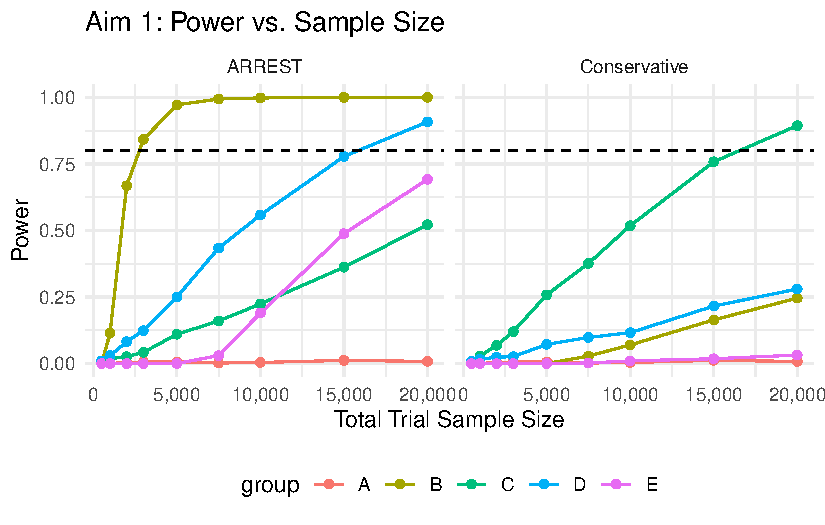
\includegraphics[keepaspectratio]{sab_hte_paper_draft_1_files/figure-pdf/tbl-aim1-table-power-1.pdf}}

}

\end{table}%

\subsubsection{Aim 2: Impact of Classification Accuracy (Post-Hoc
Analysis)}\label{aim-2-impact-of-classification-accuracy-post-hoc-analysis}

We then investigated the impact of imperfect classification accuracy on
power, bias, and error rates in a fixed, large trial of 10,000
participants. The results clearly show that decreasing accuracy has a
profoundly negative and multifaceted impact on the reliability of
post-hoc subgroup analyses.

\textbf{Power:} As shown in \texttt{Figure\ fig-aim2-plot-power},
statistical power to detect true effects diminished substantially as
classification accuracy decreased. For subgroups B and E, which had
nearly 100\% power with perfect accuracy, power fell dramatically. For
example, in Subgroup E, power dropped to below 70\% when accuracy fell
to 90\%, and to less than 20\% with 70\% accuracy. This illustrates that
even a small degree of misclassification can render a large trial
underpowered for its subgroup objectives.

\textbf{Bias:} Classification accuracy had a direct impact on the
estimation bias, as seen in \texttt{Figure\ fig-aim2-plot-bias}. For all
subgroups with a true effect (B, C, D, and E), the estimated OR was
consistently biased towards the null value of 1.0 as accuracy worsened.
This ``dilution'' effect occurs because misclassifying patients mixes
individuals from subgroups with different true effects, pulling the
observed estimate towards the population average. For example, the
powerful harmful effect in Subgroup B (OR=18.8) was severely attenuated,
with the estimated OR falling below 5.0 when accuracy dropped to 80\%.

\textbf{Wrong Direction Rate:} Perhaps most critically, the probability
of estimating an effect in the wrong direction (a Type S error)
increased as accuracy fell
(\texttt{Figure\ fig-aim2-plot-wrong-direction}). This was most
pronounced for subgroups with true effects close to the null. For the
`Conservative' scenario, where the true ORs are closer to 1.0, the
wrong-direction rate for Subgroup E was approximately 30\% even with
perfect 100\% accuracy, a consequence of the low event rate and modest
effect size. This error rate climbed to over 40\% as accuracy declined
to 70\%. This demonstrates that misclassification not only reduces the
chance of finding a true effect but also significantly increases the
risk of drawing a completely incorrect and potentially harmful
conclusion.

\begin{table}

\caption{\label{tbl-aim2-table-summary}Aim 2: Post-Hoc Analysis Summary
vs.~Accuracy (ARREST ORs, Total N = 10,000)}

\centering{

\fontsize{12.0pt}{14.4pt}\selectfont
\begin{tabular*}{\linewidth}{@{\extracolsep{\fill}}rrrrr}
\toprule
Accuracy & Power & Bias & MSE & Wrong Dir \% \\ 
\midrule\addlinespace[2.5pt]
\multicolumn{5}{l}{A} \\[2.5pt] 
\midrule\addlinespace[2.5pt]
0.50 & 3.2\% & 0.10 & 0.04 & 0.0\% \\ 
0.55 & 2.0\% & 0.09 & 0.04 & 0.0\% \\ 
0.60 & 1.6\% & 0.08 & 0.03 & 0.0\% \\ 
0.65 & 1.2\% & 0.07 & 0.03 & 0.0\% \\ 
0.70 & 1.6\% & 0.05 & 0.03 & 0.0\% \\ 
0.75 & 1.0\% & 0.04 & 0.03 & 0.0\% \\ 
0.80 & 1.0\% & 0.03 & 0.03 & 0.0\% \\ 
0.85 & 1.0\% & 0.03 & 0.03 & 0.0\% \\ 
0.90 & 0.8\% & 0.02 & 0.03 & 0.0\% \\ 
0.95 & 0.8\% & 0.00 & 0.02 & 0.0\% \\ 
0.99 & 0.4\% & -0.01 & 0.02 & 0.0\% \\ 
1.00 & 0.4\% & -0.01 & 0.02 & 0.0\% \\ 
0.50 & 1.0\% & -0.03 & 0.03 & 0.0\% \\ 
0.55 & 1.0\% & -0.02 & 0.03 & 0.0\% \\ 
0.60 & 0.8\% & -0.02 & 0.03 & 0.0\% \\ 
0.65 & 1.2\% & -0.02 & 0.03 & 0.0\% \\ 
0.70 & 1.2\% & -0.02 & 0.03 & 0.0\% \\ 
0.75 & 0.8\% & -0.02 & 0.03 & 0.0\% \\ 
0.80 & 1.4\% & -0.02 & 0.03 & 0.0\% \\ 
0.85 & 1.0\% & -0.01 & 0.03 & 0.0\% \\ 
0.90 & 0.8\% & -0.01 & 0.02 & 0.0\% \\ 
0.95 & 0.6\% & -0.01 & 0.02 & 0.0\% \\ 
0.99 & 0.4\% & -0.01 & 0.02 & 0.0\% \\ 
1.00 & 0.4\% & -0.01 & 0.02 & 0.0\% \\ 
\midrule\addlinespace[2.5pt]
\multicolumn{5}{l}{B} \\[2.5pt] 
\midrule\addlinespace[2.5pt]
0.50 & 100.0\% & -1.80 & 3.27 & 0.0\% \\ 
0.55 & 100.0\% & -1.66 & 2.82 & 0.0\% \\ 
0.60 & 100.0\% & -1.55 & 2.44 & 0.0\% \\ 
0.65 & 100.0\% & -1.43 & 2.09 & 0.0\% \\ 
0.70 & 100.0\% & -1.28 & 1.72 & 0.0\% \\ 
0.75 & 100.0\% & -1.13 & 1.36 & 0.0\% \\ 
0.80 & 100.0\% & -0.97 & 1.02 & 0.0\% \\ 
0.85 & 100.0\% & -0.79 & 0.71 & 0.0\% \\ 
0.90 & 100.0\% & -0.56 & 0.43 & 0.0\% \\ 
0.95 & 100.0\% & -0.27 & 0.24 & 0.0\% \\ 
0.99 & 100.0\% & 0.00 & 0.22 & 0.0\% \\ 
1.00 & 99.8\% & 0.11 & 0.74 & 0.0\% \\ 
0.50 & 1.2\% & -0.63 & 0.46 & 37.2\% \\ 
0.55 & 1.0\% & -0.59 & 0.43 & 37.6\% \\ 
0.60 & 1.4\% & -0.57 & 0.40 & 32.6\% \\ 
0.65 & 2.0\% & -0.54 & 0.38 & 30.2\% \\ 
0.70 & 2.2\% & -0.50 & 0.36 & 27.4\% \\ 
0.75 & 1.8\% & -0.47 & 0.34 & 24.8\% \\ 
0.80 & 3.0\% & -0.42 & 0.31 & 21.4\% \\ 
0.85 & 2.0\% & -0.37 & 0.28 & 19.0\% \\ 
0.90 & 3.8\% & -0.28 & 0.25 & 15.4\% \\ 
0.95 & 5.0\% & -0.15 & 0.26 & 11.6\% \\ 
0.99 & 6.6\% & -0.02 & 0.32 & 9.2\% \\ 
1.00 & 7.0\% & 0.06 & 0.92 & 9.0\% \\ 
\midrule\addlinespace[2.5pt]
\multicolumn{5}{l}{C} \\[2.5pt] 
\midrule\addlinespace[2.5pt]
0.50 & 0.8\% & 0.26 & 0.08 & 61.8\% \\ 
0.55 & 1.4\% & 0.24 & 0.07 & 51.0\% \\ 
0.60 & 1.2\% & 0.21 & 0.06 & 43.4\% \\ 
0.65 & 1.2\% & 0.19 & 0.05 & 36.2\% \\ 
0.70 & 1.8\% & 0.16 & 0.04 & 27.4\% \\ 
0.75 & 3.0\% & 0.14 & 0.03 & 20.0\% \\ 
0.80 & 5.8\% & 0.11 & 0.03 & 15.2\% \\ 
0.85 & 8.0\% & 0.08 & 0.02 & 10.0\% \\ 
0.90 & 12.8\% & 0.05 & 0.02 & 7.8\% \\ 
0.95 & 17.2\% & 0.02 & 0.02 & 4.6\% \\ 
0.99 & 22.2\% & 0.00 & 0.02 & 3.6\% \\ 
1.00 & 22.4\% & -0.01 & 0.02 & 3.2\% \\ 
0.50 & 14.0\% & 0.16 & 0.04 & 6.2\% \\ 
0.55 & 14.6\% & 0.14 & 0.04 & 4.6\% \\ 
0.60 & 18.2\% & 0.13 & 0.03 & 3.4\% \\ 
0.65 & 22.4\% & 0.11 & 0.03 & 2.4\% \\ 
0.70 & 25.8\% & 0.10 & 0.03 & 2.4\% \\ 
0.75 & 29.0\% & 0.08 & 0.02 & 1.2\% \\ 
0.80 & 31.8\% & 0.07 & 0.02 & 0.8\% \\ 
0.85 & 37.6\% & 0.05 & 0.02 & 0.2\% \\ 
0.90 & 42.6\% & 0.03 & 0.02 & 0.2\% \\ 
0.95 & 45.8\% & 0.01 & 0.02 & 0.2\% \\ 
0.99 & 51.0\% & 0.00 & 0.02 & 0.2\% \\ 
1.00 & 51.8\% & 0.00 & 0.02 & 0.2\% \\ 
\midrule\addlinespace[2.5pt]
\multicolumn{5}{l}{D} \\[2.5pt] 
\midrule\addlinespace[2.5pt]
0.50 & 34.2\% & -0.03 & 0.02 & 1.6\% \\ 
0.55 & 34.4\% & -0.03 & 0.02 & 1.8\% \\ 
0.60 & 38.4\% & -0.03 & 0.02 & 1.4\% \\ 
0.65 & 42.4\% & -0.03 & 0.02 & 1.4\% \\ 
0.70 & 44.0\% & -0.02 & 0.02 & 1.0\% \\ 
0.75 & 47.2\% & -0.02 & 0.02 & 0.6\% \\ 
0.80 & 49.4\% & -0.02 & 0.02 & 1.4\% \\ 
0.85 & 51.0\% & -0.01 & 0.02 & 0.8\% \\ 
0.90 & 52.2\% & -0.01 & 0.02 & 0.4\% \\ 
0.95 & 53.0\% & -0.01 & 0.02 & 0.6\% \\ 
0.99 & 54.6\% & 0.00 & 0.02 & 0.8\% \\ 
1.00 & 55.8\% & 0.00 & 0.02 & 0.8\% \\ 
0.50 & 2.8\% & -0.08 & 0.03 & 22.4\% \\ 
0.55 & 4.2\% & -0.07 & 0.03 & 22.0\% \\ 
0.60 & 3.8\% & -0.06 & 0.03 & 22.0\% \\ 
0.65 & 4.8\% & -0.05 & 0.02 & 19.2\% \\ 
0.70 & 5.8\% & -0.05 & 0.02 & 16.6\% \\ 
0.75 & 7.0\% & -0.04 & 0.02 & 15.4\% \\ 
0.80 & 7.2\% & -0.03 & 0.02 & 13.6\% \\ 
0.85 & 9.4\% & -0.02 & 0.02 & 12.8\% \\ 
0.90 & 11.0\% & -0.02 & 0.02 & 10.8\% \\ 
0.95 & 11.2\% & -0.01 & 0.02 & 8.2\% \\ 
0.99 & 11.4\% & -0.01 & 0.02 & 8.2\% \\ 
1.00 & 11.6\% & -0.01 & 0.02 & 8.4\% \\ 
\midrule\addlinespace[2.5pt]
\multicolumn{5}{l}{E} \\[2.5pt] 
\midrule\addlinespace[2.5pt]
0.50 & 2.4\% & 1.32 & 1.79 & 72.6\% \\ 
0.55 & 0.8\% & 1.29 & 1.71 & 64.2\% \\ 
0.60 & 1.2\% & 1.25 & 1.63 & 57.6\% \\ 
0.65 & 0.8\% & 1.22 & 1.55 & 52.4\% \\ 
0.70 & 0.6\% & 1.17 & 1.44 & 43.4\% \\ 
0.75 & 1.2\% & 1.10 & 1.30 & 34.6\% \\ 
0.80 & 1.2\% & 1.02 & 1.14 & 25.8\% \\ 
0.85 & 3.0\% & 0.91 & 0.96 & 21.4\% \\ 
0.90 & 5.6\% & 0.77 & 0.74 & 11.0\% \\ 
0.95 & 11.8\% & 0.50 & 0.47 & 5.2\% \\ 
0.99 & 16.6\% & 0.04 & 1.44 & 1.8\% \\ 
1.00 & 19.0\% & -0.24 & 3.72 & 1.6\% \\ 
0.50 & 1.0\% & 0.16 & 0.08 & 39.4\% \\ 
0.55 & 0.8\% & 0.14 & 0.07 & 36.4\% \\ 
0.60 & 1.2\% & 0.14 & 0.08 & 34.2\% \\ 
0.65 & 1.2\% & 0.14 & 0.08 & 37.0\% \\ 
0.70 & 0.8\% & 0.12 & 0.08 & 33.0\% \\ 
0.75 & 1.2\% & 0.11 & 0.09 & 34.0\% \\ 
0.80 & 0.8\% & 0.09 & 0.10 & 34.4\% \\ 
0.85 & 0.4\% & 0.08 & 0.11 & 33.8\% \\ 
0.90 & 1.2\% & 0.06 & 0.13 & 34.8\% \\ 
0.95 & 1.2\% & 0.02 & 0.16 & 33.0\% \\ 
0.99 & 1.2\% & -0.01 & 0.19 & 30.6\% \\ 
1.00 & 1.0\% & -0.01 & 0.21 & 30.8\% \\ 
\midrule\addlinespace[2.5pt]
\multicolumn{5}{l}{Overall} \\[2.5pt] 
\midrule\addlinespace[2.5pt]
0.50 & 95.4\% & 0.10 & 0.01 & 0.0\% \\ 
0.55 & 95.4\% & 0.10 & 0.01 & 0.0\% \\ 
0.60 & 95.4\% & 0.10 & 0.01 & 0.0\% \\ 
0.65 & 95.4\% & 0.10 & 0.01 & 0.0\% \\ 
0.70 & 95.4\% & 0.10 & 0.01 & 0.0\% \\ 
0.75 & 95.4\% & 0.10 & 0.01 & 0.0\% \\ 
0.80 & 95.4\% & 0.10 & 0.01 & 0.0\% \\ 
0.85 & 95.4\% & 0.10 & 0.01 & 0.0\% \\ 
0.90 & 95.4\% & 0.10 & 0.01 & 0.0\% \\ 
0.95 & 95.4\% & 0.10 & 0.01 & 0.0\% \\ 
0.99 & 95.4\% & 0.10 & 0.01 & 0.0\% \\ 
1.00 & 95.4\% & 0.10 & 0.01 & 0.0\% \\ 
0.50 & 8.0\% & 0.00 & 0.01 & 27.6\% \\ 
0.55 & 8.0\% & 0.00 & 0.01 & 27.6\% \\ 
0.60 & 8.0\% & 0.00 & 0.01 & 27.6\% \\ 
0.65 & 8.0\% & 0.00 & 0.01 & 27.6\% \\ 
0.70 & 8.0\% & 0.00 & 0.01 & 27.6\% \\ 
0.75 & 8.0\% & 0.00 & 0.01 & 27.6\% \\ 
0.80 & 8.0\% & 0.00 & 0.01 & 27.6\% \\ 
0.85 & 8.0\% & 0.00 & 0.01 & 27.6\% \\ 
0.90 & 8.0\% & 0.00 & 0.01 & 27.6\% \\ 
0.95 & 8.0\% & 0.00 & 0.01 & 27.6\% \\ 
0.99 & 8.0\% & 0.00 & 0.01 & 27.6\% \\ 
1.00 & 8.0\% & 0.00 & 0.01 & 27.6\% \\ 
\bottomrule
\end{tabular*}

\pandocbounded{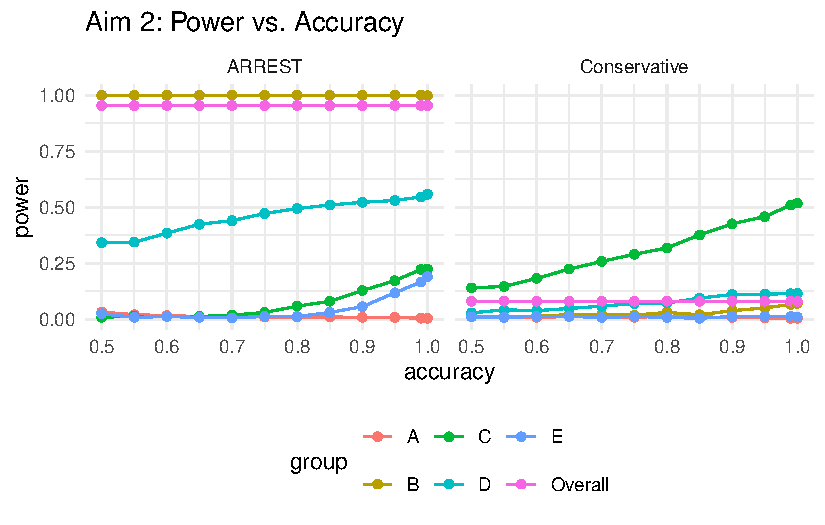
\includegraphics[keepaspectratio]{sab_hte_paper_draft_1_files/figure-pdf/tbl-aim2-table-summary-1.pdf}}

\pandocbounded{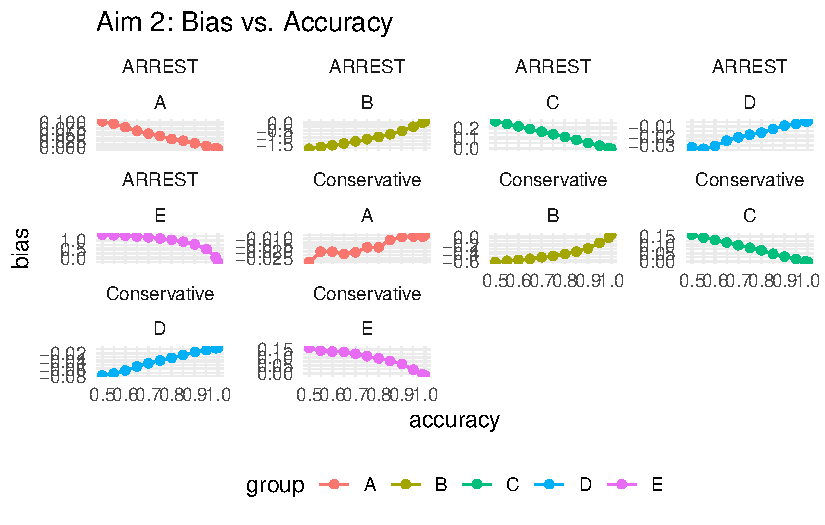
\includegraphics[keepaspectratio]{sab_hte_paper_draft_1_files/figure-pdf/tbl-aim2-table-summary-2.pdf}}

\pandocbounded{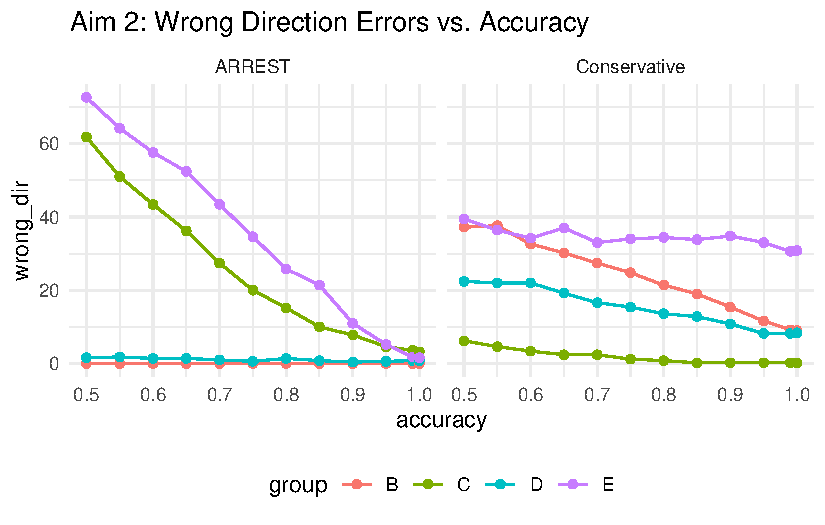
\includegraphics[keepaspectratio]{sab_hte_paper_draft_1_files/figure-pdf/tbl-aim2-table-summary-3.pdf}}

}

\end{table}%

\subsubsection{Aim 3: Sample Size Requirements (Enrichment Trial
Simulation)}\label{aim-3-sample-size-requirements-enrichment-trial-simulation}

\begin{table}

\caption{\label{tbl-aim3-nns-summary}Aim 3: Number Needed to Screen
(NNS) and Corresponding Number Needed to Randomize (NNR) to achieve 80\%
power in an enrichment trial.}

\centering{

\fontsize{12.0pt}{14.4pt}\selectfont
\begin{tabular*}{\linewidth}{@{\extracolsep{\fill}}lllr}
\toprule
Subgroup & Test Type & NNS & NNR \\ 
\midrule\addlinespace[2.5pt]
\multicolumn{4}{l}{ARREST} \\[2.5pt] 
\midrule\addlinespace[2.5pt]
B & Near-Perfect & 1,690 & 239 \\ 
B & Near-Perfect & 54,625 & 7,731 \\ 
B & High Sens/High Spec & 1,308 & 224 \\ 
B & High Sens/High Spec & 172,000 & 29,346 \\ 
B & High Sens/Low Spec & 2,718 & 1,053 \\ 
B & High Sens/Low Spec & > 1,320,000 & - \\ 
B & Low Sens/High Spec & 1,859 & 255 \\ 
B & Low Sens/High Spec & 354,000 & 48,532 \\ 
B & Balanced/Moderate & 2,819 & 791 \\ 
B & Balanced/Moderate & > 1,320,000 & - \\ 
C & Near-Perfect & 26,000 & 9,316 \\ 
C & Near-Perfect & 10,875 & 3,894 \\ 
C & High Sens/High Spec & 50,125 & 18,551 \\ 
C & High Sens/High Spec & 13,812 & 5,109 \\ 
C & High Sens/Low Spec & 176,000 & 93,477 \\ 
C & High Sens/Low Spec & 34,125 & 18,123 \\ 
C & Low Sens/High Spec & 90,250 & 25,374 \\ 
C & Low Sens/High Spec & 20,125 & 5,655 \\ 
C & Balanced/Moderate & 1,320,000 & 545,682 \\ 
C & Balanced/Moderate & 31,187 & 12,891 \\ 
D & Near-Perfect & 10,187 & 1,878 \\ 
D & Near-Perfect & 40,500 & 7,465 \\ 
D & High Sens/High Spec & 10,500 & 2,206 \\ 
D & High Sens/High Spec & 51,500 & 10,824 \\ 
D & High Sens/Low Spec & 8,750 & 3,635 \\ 
D & High Sens/Low Spec & 241,500 & 100,356 \\ 
D & Low Sens/High Spec & 14,968 & 2,479 \\ 
D & Low Sens/High Spec & 78,250 & 12,963 \\ 
D & Balanced/Moderate & 11,562 & 3,549 \\ 
D & Balanced/Moderate & 183,500 & 56,280 \\ 
E & Near-Perfect & 36,125 & 6,655 \\ 
E & Near-Perfect & 330,000 & 60,809 \\ 
E & High Sens/High Spec & 566,000 & 118,879 \\ 
E & High Sens/High Spec & 546,000 & 114,676 \\ 
E & High Sens/Low Spec & 31,125 & 12,934 \\ 
E & High Sens/Low Spec & 580,000 & 241,044 \\ 
E & Low Sens/High Spec & > 1,320,000 & - \\ 
E & Low Sens/High Spec & 802,000 & 132,822 \\ 
E & Balanced/Moderate & 56,000 & 17,170 \\ 
E & Balanced/Moderate & 704,000 & 215,930 \\ 
\midrule\addlinespace[2.5pt]
\multicolumn{4}{l}{Conservative} \\[2.5pt] 
\midrule\addlinespace[2.5pt]
B & Near-Perfect & 1,690 & 239 \\ 
B & Near-Perfect & 54,625 & 7,731 \\ 
B & High Sens/High Spec & 1,308 & 224 \\ 
B & High Sens/High Spec & 172,000 & 29,346 \\ 
B & High Sens/Low Spec & 2,718 & 1,053 \\ 
B & High Sens/Low Spec & > 1,320,000 & - \\ 
B & Low Sens/High Spec & 1,859 & 255 \\ 
B & Low Sens/High Spec & 354,000 & 48,532 \\ 
B & Balanced/Moderate & 2,819 & 791 \\ 
B & Balanced/Moderate & > 1,320,000 & - \\ 
C & Near-Perfect & 26,000 & 9,316 \\ 
C & Near-Perfect & 10,875 & 3,894 \\ 
C & High Sens/High Spec & 50,125 & 18,551 \\ 
C & High Sens/High Spec & 13,812 & 5,109 \\ 
C & High Sens/Low Spec & 176,000 & 93,477 \\ 
C & High Sens/Low Spec & 34,125 & 18,123 \\ 
C & Low Sens/High Spec & 90,250 & 25,374 \\ 
C & Low Sens/High Spec & 20,125 & 5,655 \\ 
C & Balanced/Moderate & 1,320,000 & 545,682 \\ 
C & Balanced/Moderate & 31,187 & 12,891 \\ 
D & Near-Perfect & 10,187 & 1,878 \\ 
D & Near-Perfect & 40,500 & 7,465 \\ 
D & High Sens/High Spec & 10,500 & 2,206 \\ 
D & High Sens/High Spec & 51,500 & 10,824 \\ 
D & High Sens/Low Spec & 8,750 & 3,635 \\ 
D & High Sens/Low Spec & 241,500 & 100,356 \\ 
D & Low Sens/High Spec & 14,968 & 2,479 \\ 
D & Low Sens/High Spec & 78,250 & 12,963 \\ 
D & Balanced/Moderate & 11,562 & 3,549 \\ 
D & Balanced/Moderate & 183,500 & 56,280 \\ 
E & Near-Perfect & 36,125 & 6,655 \\ 
E & Near-Perfect & 330,000 & 60,809 \\ 
E & High Sens/High Spec & 566,000 & 118,879 \\ 
E & High Sens/High Spec & 546,000 & 114,676 \\ 
E & High Sens/Low Spec & 31,125 & 12,934 \\ 
E & High Sens/Low Spec & 580,000 & 241,044 \\ 
E & Low Sens/High Spec & > 1,320,000 & - \\ 
E & Low Sens/High Spec & 802,000 & 132,822 \\ 
E & Balanced/Moderate & 56,000 & 17,170 \\ 
E & Balanced/Moderate & 704,000 & 215,930 \\ 
\bottomrule
\end{tabular*}

\pandocbounded{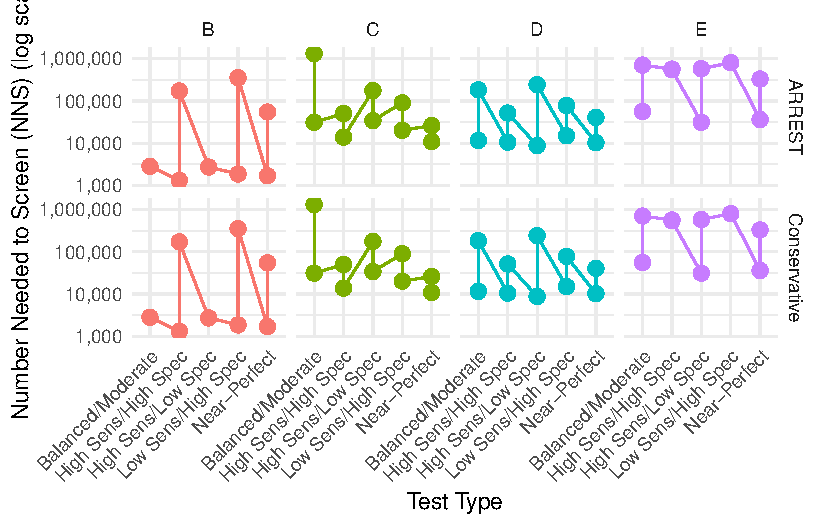
\includegraphics[keepaspectratio]{sab_hte_paper_draft_1_files/figure-pdf/tbl-aim3-nns-summary-1.pdf}}

\pandocbounded{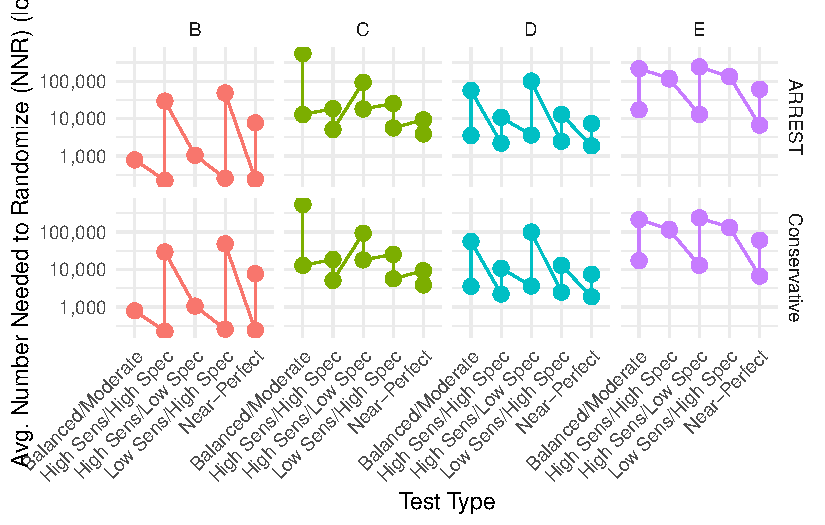
\includegraphics[keepaspectratio]{sab_hte_paper_draft_1_files/figure-pdf/tbl-aim3-nns-summary-2.pdf}}

}

\end{table}%

\section{Discussion}\label{discussion}

This simulation study demonstrates the significant challenges in
detecting heterogeneous treatment effects in the presence of subgroup
misclassification, using parameters derived from a real-world \emph{S.
aureus} bacteremia trial (5).

\subsubsection{Strengths and
Limitations}\label{strengths-and-limitations}

A key strength of this study is its grounding in a real-world clinical
problem, using parameters from a well-characterized cohort to ensure the
data-generating mechanisms are as plausible as possible. The systematic,
multi-aim structure, following the ADEMP framework, provides a
comprehensive view of the problem from foundational power calculations
to the practical implications for enrichment trial design.

However, our study has several limitations inherent to any simulation
work. Our misclassification model assumes that when an error occurs, the
assigned subgroup is chosen randomly according to population prevalence.
This represents a scenario where a diagnostic provides no information
upon failure. In reality, misclassifications may not be random; for
instance, two clinically similar subgroups may be more frequently
confused for one another. A more complex model using a pre-defined
confusion matrix could explore such scenarios, representing a potential
avenue for future research.

Furthermore, while the ``Realistic Scenario'' provides a valuable
sensitivity analysis, the chosen moderate ORs are illustrative. The true
extent of HTE in SAB is still unknown, and future work could explore a
wider range of effect sizes to create a broader map of the statistical
challenges. Finally, our simulations do not account for other real-world
complexities such as variability in diagnostic accuracy across sites or
over time.

Aim 1 highlights that even with perfect classification, substantial
sample sizes are required to achieve adequate power (80\%) for
\textbf{post-hoc subgroup analyses} within a standard trial randomizing
the full population mix (\textbf{?@fig-aim1-plot-power}). This is
particularly true for less prevalent subgroups or those with smaller
effect sizes, or where baseline event rates are low (even if the
relative effect is large, as seen for subgroup B with the ARREST
parameters). The need for multiple comparison adjustments (e.g.,
Bonferroni) further inflates sample size requirements for post-hoc
analyses (10).

Aim 2 quantifies the detrimental impact of misclassification accuracy on
these post-hoc analyses (\textbf{?@fig-aim2-plot-power},
\textbf{?@fig-aim2-plot-bias},
\textbf{?@fig-aim2-plot-wrong-direction}). As accuracy decreases,
statistical power diminishes substantially, bias in effect estimates
increases (generally towards the overall null effect), and the
probability of estimating effects in the wrong direction rises. This
underscores the critical importance of highly accurate subgroup
classification methods if relying on post-hoc analyses and aligns with
broader concerns about the reliability of subgroup findings {[}(11);
Kent2018{]}. Subgroups with true null effects (like A) are particularly
susceptible to high rates of ``wrong direction'' findings under
misclassification.

\subsubsection{Practical Implications: Enrichment
Trials}\label{practical-implications-enrichment-trials}

Aim 3 simulates an \textbf{enrichment trial} design, where patients are
screened using a test with a given \texttt{accuracy} (probability of
correct classification), and only those testing positive for the target
subgroup are randomized. This allows estimation of the Number Needed to
Screen (NNS) and the average resulting Number Needed to Randomize
(NNREnrich) within the enriched cohort required to achieve 80\% power.

The results (\textbf{?@tbl-implications-table},
\textbf{?@fig-aim3-plot-power}, \textbf{?@fig-aim3-plot-nns})
demonstrate the trade-offs inherent in enrichment designs {[}(12);
Antoniou2016{]}. While potentially requiring fewer randomized patients
(NNR) compared to the total N needed for post-hoc power (Aim 1), the
screening burden (NNS) can be substantial and increases dramatically as
test accuracy decreases. For example, achieving 80\% power for subgroup
B (OR=18.8) requires screening tens of thousands even with high
accuracy, due to its prevalence and the corrected baseline risk. Lower
accuracy inflates NNR (due to dilution by false positives) and NNS (due
to lower yield). This highlights that the feasibility of enrichment
trials depends critically on subgroup prevalence, effect size, and,
crucially, the performance characteristics of the screening test {[}(8);
Wang2014{]}. Our simulations using more realistic ORs show lower, more
achievable NNR/NNS values (see
\textbf{?@tbl-implications-table-realistic} and
\textbf{?@fig-aim3-plot-nnr-nns-realistic}), but the strong dependence
on accuracy remains.

\subsection{Conclusion}\label{conclusion}

This simulation study underscores the importance of considering
classification accuracy when interpreting subgroup analyses or planning
trials aimed at detecting HTE in heterogeneous diseases like SAB.
Post-hoc subgroup analyses require large sample sizes and high
classification accuracy to yield reliable results. Enrichment trial
designs offer potential efficiency gains in terms of randomized patients
but necessitate careful evaluation of the screening burden, which is
highly sensitive to test accuracy and subgroup prevalence. Developing
and validating accurate methods for identifying SAB subphenotypes is
crucial for advancing stratified medicine approaches in this field.

\subsection{References}\label{references}

\emph{(Ensure references.bib and vancouver.csl are in the same directory
or provide correct paths)}

\begin{Shaded}
\begin{Highlighting}[]
\VariableTok{@article}\NormalTok{\{}\OtherTok{Swets2024}\NormalTok{,}
  \DataTypeTok{author}\NormalTok{ = \{Swets, Maaike C and Bakk, Zsuzsa and Westgeest, Annette C and Berry, Karla and Cooper, George and Sim, Wynne and Lee, Rui Shian and Gan, Tze Yi and Donlon, William and Besu, Antonia and Heppenstall, Ellen and Tysall, Lauren and Dewar, Scott and de Boer, Mark G J and Fowler, Jr, Vance G and Dockrell, David H and Thwaites, Guy E and Pujol, Miquel and Pallares, Nuria and Tebe, Cristòfol and Carratalà, Jordi and Szubert, Alan J and Groeneveld, G H Rolf and Russell, Clark D\},}
  \DataTypeTok{year}\NormalTok{ = \{2024\},}
  \DataTypeTok{month}\NormalTok{ = \{06\},}
  \DataTypeTok{pages}\NormalTok{ = \{1153{-}1161\},}
  \DataTypeTok{title}\NormalTok{ = \{Clinical Subphenotypes of Staphylococcus aureus Bacteremia\},}
  \DataTypeTok{volume}\NormalTok{ = \{79\},}
  \DataTypeTok{journal}\NormalTok{ = \{Clinical Infectious Diseases\},}
  \DataTypeTok{doi}\NormalTok{ = \{10.1093/cid/ciae338\}}
\NormalTok{\}}

\VariableTok{@article}\NormalTok{\{}\OtherTok{Morris2019}\NormalTok{,}
    \DataTypeTok{author}\NormalTok{ = \{Morris, Tim P. and White, Ian R. and Crowther, Michael J.\},}
    \DataTypeTok{title}\NormalTok{ = "}\StringTok{\{Using simulation studies to evaluate statistical methods\}}\NormalTok{",}
    \DataTypeTok{journal}\NormalTok{ = \{Statistics in Medicine\},}
    \DataTypeTok{volume}\NormalTok{ = \{38\},}
    \DataTypeTok{number}\NormalTok{ = \{11\},}
    \DataTypeTok{pages}\NormalTok{ = \{2074{-}2102\},}
    \DataTypeTok{keywords}\NormalTok{ = \{Monte Carlo, reporting guideline, simulation study, statistical methods\},}
    \DataTypeTok{doi}\NormalTok{ = \{https://doi.org/10.1002/sim.8086\},}
    \DataTypeTok{url}\NormalTok{ = \{https://onlinelibrary.wiley.com/doi/abs/10.1002/sim.8086\},}
    \DataTypeTok{eprint}\NormalTok{ = \{https://onlinelibrary.wiley.com/doi/pdf/10.1002/sim.8086\},}
    \DataTypeTok{year}\NormalTok{ = \{2019\}}
\NormalTok{\}}

\VariableTok{@article}\NormalTok{\{}\OtherTok{Siepe2024}\NormalTok{,}
    \DataTypeTok{year}\NormalTok{ = \{2024\},}
    \DataTypeTok{author}\NormalTok{ = \{Björn S. Siepe and František Bartoš and Tim P. Morris and Anne{-}Laure Boulesteix and Daniel W. Heck and Samuel Pawel\},}
    \DataTypeTok{title}\NormalTok{ = \{Simulation Studies for Methodological Research in Psychology: A Standardized Structure for Planning, Preregistration, and Reporting\},}
    \DataTypeTok{doi}\NormalTok{ = \{10.1037/met0000695\},}
    \DataTypeTok{url}\NormalTok{ = \{https://doi.org/10.1037/met0000695\},}
    \DataTypeTok{journal}\NormalTok{ = \{Psychological Methods\}}
\NormalTok{\}}

\VariableTok{@article}\NormalTok{\{}\OtherTok{Tong2015}\NormalTok{,}
    \DataTypeTok{author}\NormalTok{ = \{Tong, Steven Y. C. and Davis, Joshua S. and Eichenberger, Emily and Holland, Thomas L. and Fowler, Vance G.\},}
    \DataTypeTok{title}\NormalTok{ = "}\StringTok{\{Staphylococcus aureus Infections: Epidemiology, Pathophysiology, Clinical Manifestations, and Management\}}\NormalTok{",}
    \DataTypeTok{journal}\NormalTok{ = \{Clinical Microbiology Reviews\},}
    \DataTypeTok{volume}\NormalTok{ = \{28\},}
    \DataTypeTok{number}\NormalTok{ = \{3\},}
    \DataTypeTok{pages}\NormalTok{ = \{603{-}661\},}
    \DataTypeTok{year}\NormalTok{ = \{2015\},}
    \DataTypeTok{doi}\NormalTok{ = \{10.1128/CMR.00134{-}14\},}
    \DataTypeTok{url}\NormalTok{ = \{https://journals.asm.org/doi/abs/10.1128/CMR.00134{-}14\}}
\NormalTok{\}}

\VariableTok{@article}\NormalTok{\{}\OtherTok{GBD2019}\NormalTok{,}
    \DataTypeTok{author}\NormalTok{ = \{\{GBD 2019 Antimicrobial Resistance Collaborators\}\},}
    \DataTypeTok{title}\NormalTok{ = "}\StringTok{\{Global mortality associated with 33 bacterial pathogens in 2019: a systematic analysis for the Global Burden of Disease Study 2019\}}\NormalTok{",}
    \DataTypeTok{journal}\NormalTok{ = \{The Lancet\},}
    \DataTypeTok{volume}\NormalTok{ = \{400\},}
    \DataTypeTok{number}\NormalTok{ = \{10369\},}
    \DataTypeTok{pages}\NormalTok{ = \{2221{-}2248\},}
    \DataTypeTok{year}\NormalTok{ = \{2022\},}
    \DataTypeTok{doi}\NormalTok{ = \{10.1016/S0140{-}6736(22)02185{-}7\}}
\NormalTok{\}}

\VariableTok{@article}\NormalTok{\{}\OtherTok{Thwaites2018}\NormalTok{,}
    \DataTypeTok{author}\NormalTok{ = \{Thwaites, Guy E. and Scarborough, Matthew and Szubert, Alan and Nsutebu, Emmanuel and Tilley, Richard and Greig, Jane and Wyllie, Sarah A. and Wilson, Peter and Auckland, Chloë and Cairns, John and Ward, Debbi and Lal, Punam and Barlow, Gavin and Hopkins, Susan and Gkrania{-}Klotsas, Effrossyni Z. and Shankaran, Padmasarda and Cripps, Natasha and Davies, Jonathan and Harvey, David and Gubbay, Andrew J. and Klein, J. Louis and Bradley, Chris and Morgan, Mari and Llewelyn, Martin J. and Edgeworth, Jonathan D. and Walker, A. Sarah\},}
    \DataTypeTok{title}\NormalTok{ = "}\StringTok{\{Adjunctive rifampicin for Staphylococcus aureus bacteraemia (ARREST): a multicentre, randomised, double{-}blind, placebo{-}controlled trial\}}\NormalTok{",}
    \DataTypeTok{journal}\NormalTok{ = \{The Lancet\},}
    \DataTypeTok{volume}\NormalTok{ = \{391\},}
    \DataTypeTok{number}\NormalTok{ = \{10121\},}
    \DataTypeTok{pages}\NormalTok{ = \{668{-}678\},}
    \DataTypeTok{year}\NormalTok{ = \{2018\},}
    \DataTypeTok{doi}\NormalTok{ = \{10.1016/S0140{-}6736(17)32446{-}X\}}
\NormalTok{\}}

\VariableTok{@article}\NormalTok{\{}\OtherTok{Holland2022}\NormalTok{,}
    \DataTypeTok{author}\NormalTok{ = \{Holland, Thomas L. and Bayer, Arnold S. and Fowler, Vance G.\},}
    \DataTypeTok{title}\NormalTok{ = "}\StringTok{\{Persistent Staphylococcus aureus Bacteremia: Challenges and Controversies\}}\NormalTok{",}
    \DataTypeTok{journal}\NormalTok{ = \{Clinical Infectious Diseases\},}
    \DataTypeTok{volume}\NormalTok{ = \{75\},}
    \DataTypeTok{number}\NormalTok{ = \{10\},}
    \DataTypeTok{pages}\NormalTok{ = \{1863{-}1870\},}
    \DataTypeTok{year}\NormalTok{ = \{2022\},}
    \DataTypeTok{doi}\NormalTok{ = \{10.1093/cid/ciac4 persistent\}}
\NormalTok{\}}

\VariableTok{@article}\NormalTok{\{}\OtherTok{Paulsen2024}\NormalTok{,}
    \DataTypeTok{author}\NormalTok{ = \{Paulsen, Johann and Giske, Christian G. and Frimodt{-}Møller, Niels and Knudsen, Jenny Dahl and Petersen, Andreas and Kjøbek, Lotte and Brandt, Carolin and Jensen, Uffe S. and Schønheyder, Henrik C. and Knudsen, Ida D. and Østergaard, Christian and Arpi, Magnus and Andersen, Claus and Tønder, Rikke V. and Søndergaard, Tove S. and Rosenvinge, Flemming S. and Møller, Jacob K. and Jensen, Thøger G. and Kjær, Jacob and Lindegaard, Bente and Benfield, Thomas\},}
    \DataTypeTok{title}\NormalTok{ = "}\StringTok{\{Ceftaroline vs Standard{-}of{-}Care Antibiotics for Treatment of Complicated Staphylococcus aureus Bacteremia: A Randomized Clinical Trial\}}\NormalTok{",}
    \DataTypeTok{journal}\NormalTok{ = \{JAMA Internal Medicine\},}
    \DataTypeTok{volume}\NormalTok{ = \{184\},}
    \DataTypeTok{number}\NormalTok{ = \{2\},}
    \DataTypeTok{pages}\NormalTok{ = \{143{-}151\},}
    \DataTypeTok{year}\NormalTok{ = \{2024\},}
    \DataTypeTok{doi}\NormalTok{ = \{10.1001/jamainternmed.2023.6764\}}
\NormalTok{\}}

\VariableTok{@article}\NormalTok{\{}\OtherTok{Davis2023}\NormalTok{,}
    \DataTypeTok{author}\NormalTok{ = \{Davis, Joshua S. and Stevens, Vanessa and van Hal, Sebastiaan J.\},}
    \DataTypeTok{title}\NormalTok{ = "}\StringTok{\{Time to get personal with Staphylococcus aureus bacteraemia\}}\NormalTok{",}
    \DataTypeTok{journal}\NormalTok{ = \{Clinical Microbiology and Infection\},}
    \DataTypeTok{volume}\NormalTok{ = \{29\},}
    \DataTypeTok{number}\NormalTok{ = \{11\},}
    \DataTypeTok{pages}\NormalTok{ = \{1357{-}1359\},}
    \DataTypeTok{year}\NormalTok{ = \{2023\},}
    \DataTypeTok{doi}\NormalTok{ = \{https://doi.org/10.1016/j.cmi.2023.07.017\}}
\NormalTok{\}}

\VariableTok{@article}\NormalTok{\{}\OtherTok{Siontis2014}\NormalTok{,}
    \DataTypeTok{author}\NormalTok{ = \{Siontis, George C.M. and Tzoulaki, Ioanna and Castaldi, Peter J. and Ioannidis, John P.A.\},}
    \DataTypeTok{title}\NormalTok{ = "}\StringTok{\{External validation of new risk prediction models is infrequent and reveals worse prognostic discrimination\}}\NormalTok{",}
    \DataTypeTok{journal}\NormalTok{ = \{Journal of Clinical Epidemiology\},}
    \DataTypeTok{volume}\NormalTok{ = \{68\},}
    \DataTypeTok{number}\NormalTok{ = \{1\},}
    \DataTypeTok{pages}\NormalTok{ = \{25{-}34\},}
    \DataTypeTok{year}\NormalTok{ = \{2015\},}
    \DataTypeTok{doi}\NormalTok{ = \{https://doi.org/10.1016/j.jclinepi.2014.09.007\}}
\NormalTok{\}}

\VariableTok{@article}\NormalTok{\{}\OtherTok{Kent2018}\NormalTok{,}
    \DataTypeTok{author}\NormalTok{ = \{Kent, David M. and Steyerberg, Ewout W. and van Klaveren, David\},}
    \DataTypeTok{title}\NormalTok{ = "}\StringTok{\{Personalized evidence based medicine: predictive approaches to heterogeneous treatment effects\}}\NormalTok{",}
    \DataTypeTok{journal}\NormalTok{ = \{BMJ\},}
    \DataTypeTok{volume}\NormalTok{ = \{363\},}
    \DataTypeTok{pages}\NormalTok{ = \{k4245\},}
    \DataTypeTok{year}\NormalTok{ = \{2018\},}
    \DataTypeTok{doi}\NormalTok{ = \{10.1136/bmj.k4245\}}
\NormalTok{\}}

\VariableTok{@article}\NormalTok{\{}\OtherTok{Sussman2017}\NormalTok{,}
    \DataTypeTok{author}\NormalTok{ = \{Sussman, Jeremy B. and Hayward, Rodney A.\},}
    \DataTypeTok{title}\NormalTok{ = "}\StringTok{\{An IV for the Use of Subgroup Analysis in Randomized Trials\}}\NormalTok{",}
    \DataTypeTok{journal}\NormalTok{ = \{Annals of Internal Medicine\},}
    \DataTypeTok{volume}\NormalTok{ = \{153\},}
    \DataTypeTok{number}\NormalTok{ = \{2\},}
    \DataTypeTok{pages}\NormalTok{ = \{124{-}130\},}
    \DataTypeTok{year}\NormalTok{ = \{2010\},}
    \DataTypeTok{doi}\NormalTok{ = \{10.7326/0003{-}4819{-}153{-}2{-}201007200{-}00263\}}
\NormalTok{\}}

\VariableTok{@article}\NormalTok{\{}\OtherTok{Anthenelli2011}\NormalTok{,}
    \DataTypeTok{author}\NormalTok{ = \{Anthenelli, Robert M. and Simon, Neal and O\textquotesingle{}Malley, Stephanie S. and Breslow, Roger and West, Robert and McRee, Bud and Hoffmann, David and Interpol, Claire and Meyer, Roger and Simon, Richard\},}
    \DataTypeTok{title}\NormalTok{ = "}\StringTok{\{An Evaluation of the Use of Biomarkers to Predict the Effects of Varenicline on Smoking Cessation and Safety\}}\NormalTok{",}
    \DataTypeTok{journal}\NormalTok{ = \{Annals of Internal Medicine\},}
    \DataTypeTok{volume}\NormalTok{ = \{155\},}
    \DataTypeTok{number}\NormalTok{ = \{11\},}
    \DataTypeTok{pages}\NormalTok{ = \{760{-}771\},}
    \DataTypeTok{year}\NormalTok{ = \{2011\},}
    \DataTypeTok{doi}\NormalTok{ = \{10.7326/0003{-}4819{-}155{-}11{-}201112060{-}00007\}}
\NormalTok{\}}

\VariableTok{@article}\NormalTok{\{}\OtherTok{Simon2004}\NormalTok{,}
    \DataTypeTok{author}\NormalTok{ = \{Simon, Richard and Maitournam, Aboubakar\},}
    \DataTypeTok{title}\NormalTok{ = "}\StringTok{\{Evaluating the efficiency of targeted designs for randomized clinical trials\}}\NormalTok{",}
    \DataTypeTok{journal}\NormalTok{ = \{Clinical Cancer Research\},}
    \DataTypeTok{volume}\NormalTok{ = \{10\},}
    \DataTypeTok{number}\NormalTok{ = \{19\},}
    \DataTypeTok{pages}\NormalTok{ = \{6759{-}6763\},}
    \DataTypeTok{year}\NormalTok{ = \{2004\},}
    \DataTypeTok{doi}\NormalTok{ = \{10.1158/1078{-}0432.CCR{-}04{-}0721\}}
\NormalTok{\}}

\VariableTok{@article}\NormalTok{\{}\OtherTok{Wang2007}\NormalTok{,}
    \DataTypeTok{author}\NormalTok{ = \{Wang, Rong and Lagakos, Stephen W. and Ware, James H. and Hunter, David J. and Drazen, Jeffrey M.\},}
    \DataTypeTok{title}\NormalTok{ = "}\StringTok{\{Statistics in Medicine — Reporting of Subgroup Analyses in Clinical Trials\}}\NormalTok{",}
    \DataTypeTok{journal}\NormalTok{ = \{New England Journal of Medicine\},}
    \DataTypeTok{volume}\NormalTok{ = \{357\},}
    \DataTypeTok{number}\NormalTok{ = \{21\},}
    \DataTypeTok{pages}\NormalTok{ = \{2189{-}2194\},}
    \DataTypeTok{year}\NormalTok{ = \{2007\},}
    \DataTypeTok{doi}\NormalTok{ = \{10.1056/NEJMsr077003\}}
\NormalTok{\}}

\VariableTok{@article}\NormalTok{\{}\OtherTok{Pocock2007}\NormalTok{,}
    \DataTypeTok{author}\NormalTok{ = \{Pocock, Stuart J. and Assmann, Susan E. and Enos, Lori E. and Kasten, Linda E.\},}
    \DataTypeTok{title}\NormalTok{ = "}\StringTok{\{Subgroup analysis, covariate adjustment and baseline comparisons in clinical trial reporting: current practice and problems\}}\NormalTok{",}
    \DataTypeTok{journal}\NormalTok{ = \{Statistics in Medicine\},}
    \DataTypeTok{volume}\NormalTok{ = \{21\},}
    \DataTypeTok{number}\NormalTok{ = \{19\},}
    \DataTypeTok{pages}\NormalTok{ = \{2917{-}2930\},}
    \DataTypeTok{year}\NormalTok{ = \{2002\},}
    \DataTypeTok{doi}\NormalTok{ = \{https://doi.org/10.1002/sim.1296\}}
\NormalTok{\}}

\VariableTok{@article}\NormalTok{\{}\OtherTok{Antoniou2016}\NormalTok{,}
    \DataTypeTok{author}\NormalTok{ = \{Antoniou, Michael and Jorgensen, Andrea L. and Kolamunnage{-}Dona, Ruwanthi\},}
    \DataTypeTok{title}\NormalTok{ = "}\StringTok{\{Biomarker{-}guided adaptive enrichment designs in clinical trials: A review of methods and challenges\}}\NormalTok{",}
    \DataTypeTok{journal}\NormalTok{ = \{Contemporary Clinical Trials\},}
    \DataTypeTok{volume}\NormalTok{ = \{48\},}
    \DataTypeTok{pages}\NormalTok{ = \{104{-}114\},}
    \DataTypeTok{year}\NormalTok{ = \{2016\},}
    \DataTypeTok{doi}\NormalTok{ = \{https://doi.org/10.1016/j.cct.2016.04.006\}}
\NormalTok{\}}

\VariableTok{@article}\NormalTok{\{}\OtherTok{Wang2014}\NormalTok{,}
    \DataTypeTok{author}\NormalTok{ = \{Wang, Sue{-}Jane and Hung, H. M. James and O\textquotesingle{}Neill, Robert T.\},}
    \DataTypeTok{title}\NormalTok{ = "}\StringTok{\{Adaptive enrichment trial design challenges and opportunities\}}\NormalTok{",}
    \DataTypeTok{journal}\NormalTok{ = \{Biometrical Journal\},}
    \DataTypeTok{volume}\NormalTok{ = \{56\},}
    \DataTypeTok{number}\NormalTok{ = \{1\},}
    \DataTypeTok{pages}\NormalTok{ = \{146{-}161\},}
    \DataTypeTok{year}\NormalTok{ = \{2014\},}
    \DataTypeTok{doi}\NormalTok{ = \{https://doi.org/10.1002/bimj.201300158\}}
\NormalTok{\}}
\end{Highlighting}
\end{Shaded}

\section{Supplementary Material}\label{supplementary-material}

\#\textbar{} label: fig-supp-bias-arrest \#\textbar{} fig-cap: ``Bias
Distribution vs Accuracy (ARREST ORs, N = 10,000). Bias calculated
against target log(OR) for each group label.''

\section{Plotting bias\_val which compares estimated beta to
true\_beta\_target}\label{plotting-bias_val-which-compares-estimated-beta-to-true_beta_target}

if (exists(``results\_aim2\_processed'') \&\&
nrow(results\_aim2\_processed) \textgreater{} 0) \{ \# Filter out
Overall group for this plot ggplot(results\_aim2\_processed
\%\textgreater\% filter(group != ``Overall''), aes(x = factor(accuracy),
y = bias\_val, fill = group)) + \# Use boxplot to show distribution of
bias geom\_boxplot(position = position\_dodge(width = 0.7),
outlier.shape = NA) + \# Hide outliers for clarity \# Add horizontal
line at zero bias for reference geom\_hline(yintercept = 0, linetype =
``dashed'', color = ``black'') + facet\_wrap(\textasciitilde{} group,
scales = ``free\_y'') + \# Separate plot per subgroup labs( \# title =
paste(``Bias Distribution vs Accuracy (ARREST; n ='', n\_fixed\_aim2,
``)''), \# Redundant \# subtitle = ``Bias calculated against target
log(OR) for each group label'', x = ``Classification Accuracy'', y =
``Bias (log OR)'' ) + theme(axis.text.x = element\_text(angle = 45,
hjust = 1), legend.position = ``none'') \# Hide redundant legend \} else
\{ print(``Data frame `results\_aim2\_processed' not found or is empty.
Cannot generate supplementary bias plot for ARREST ORs.'') \}
\#\textbar{} label: fig-supp-bias-realistic \#\textbar{} fig-cap: ``Bias
Distribution vs Accuracy (Realistic ORs, N = 10,000). Bias calculated
against target log(OR) for each group label.''

\section{Plotting bias\_val for realistic
scenario}\label{plotting-bias_val-for-realistic-scenario}

if (exists(``results\_aim2\_real\_processed'') \&\&
nrow(results\_aim2\_real\_processed) \textgreater{} 0) \{ \# Filter out
Overall group ggplot(results\_aim2\_real\_processed \%\textgreater\%
filter(group != ``Overall''), aes(x = factor(accuracy), y = bias\_val,
fill = group)) + geom\_boxplot(position = position\_dodge(width = 0.7),
outlier.shape = NA) + \# Hide outliers \# Hline at zero bias
geom\_hline(yintercept = 0, linetype = ``dashed'', color = ``black'') +
facet\_wrap(\textasciitilde{} group, scales = ``free\_y'') + labs( \#
title = paste(``Bias Distribution vs Accuracy (Realistic; n ='',
n\_fixed\_aim2, ``)''), \# Redundant \# subtitle = ``Bias calculated
against target log(OR) for each group label'', x = ``Classification
Accuracy'', y = ``Bias (log OR)'' ) + theme(axis.text.x =
element\_text(angle = 45, hjust = 1), legend.position = ``none'') \#
Hide redundant legend \} else \{ print(``Data frame
`results\_aim2\_real\_processed' not found or is empty. Cannot generate
supplementary bias plot for Realistic ORs.'') \} ```qmd

\phantomsection\label{refs}
\begin{CSLReferences}{0}{1}
\bibitem[\citeproctext]{ref-Tong2015}
\CSLLeftMargin{1. }%
\CSLRightInline{Tong SYC, Davis JS, Eichenberger E, Holland TL, Fowler
VG. {Staphylococcus aureus Infections: Epidemiology, Pathophysiology,
Clinical Manifestations, and Management}. Clinical Microbiology Reviews
{[}Internet{]}. 2015;28(3):603--61. Available from:
\url{https://journals.asm.org/doi/abs/10.1128/CMR.00134-14}}

\bibitem[\citeproctext]{ref-GBD2019}
\CSLLeftMargin{2. }%
\CSLRightInline{GBD 2019 Antimicrobial Resistance Collaborators.
\href{https://doi.org/10.1016/S0140-6736(22)02185-7}{{Global mortality
associated with 33 bacterial pathogens in 2019: a systematic analysis
for the Global Burden of Disease Study 2019}}. The Lancet.
2022;400(10369):2221--48. }

\bibitem[\citeproctext]{ref-Thwaites2018}
\CSLLeftMargin{3. }%
\CSLRightInline{Thwaites GE, Scarborough M, Szubert A, Nsutebu E, Tilley
R, Greig J, et al.
\href{https://doi.org/10.1016/S0140-6736(17)32446-X}{{Adjunctive
rifampicin for Staphylococcus aureus bacteraemia (ARREST): a
multicentre, randomised, double-blind, placebo-controlled trial}}. The
Lancet. 2018;391(10121):668--78. }

\bibitem[\citeproctext]{ref-Davis2023}
\CSLLeftMargin{4. }%
\CSLRightInline{Davis JS, Stevens V, Hal SJ van.
\href{https://doi.org/10.1016/j.cmi.2023.07.017}{{Time to get personal
with Staphylococcus aureus bacteraemia}}. Clinical Microbiology and
Infection. 2023;29(11):1357--9. }

\bibitem[\citeproctext]{ref-Swets2024}
\CSLLeftMargin{5. }%
\CSLRightInline{Swets MC, Bakk Z, Westgeest AC, Berry K, Cooper G, Sim
W, et al. \href{https://doi.org/10.1093/cid/ciae338}{Clinical
subphenotypes of staphylococcus aureus bacteremia}. Clinical Infectious
Diseases. 2024 Jun;79:1153--61. }

\bibitem[\citeproctext]{ref-Siontis2014}
\CSLLeftMargin{6. }%
\CSLRightInline{Siontis GCM, Tzoulaki I, Castaldi PJ, Ioannidis JPA.
\href{https://doi.org/10.1016/j.jclinepi.2014.09.007}{{External
validation of new risk prediction models is infrequent and reveals worse
prognostic discrimination}}. Journal of Clinical Epidemiology.
2015;68(1):25--34. }

\bibitem[\citeproctext]{ref-Kent2018}
\CSLLeftMargin{7. }%
\CSLRightInline{Kent DM, Steyerberg EW, Klaveren D van.
\href{https://doi.org/10.1136/bmj.k4245}{{Personalized evidence based
medicine: predictive approaches to heterogeneous treatment effects}}.
BMJ. 2018;363:k4245. }

\bibitem[\citeproctext]{ref-Anthenelli2011}
\CSLLeftMargin{8. }%
\CSLRightInline{Anthenelli RM, Simon N, O'Malley SS, Breslow R, West R,
McRee B, et al.
\href{https://doi.org/10.7326/0003-4819-155-11-201112060-00007}{{An
Evaluation of the Use of Biomarkers to Predict the Effects of
Varenicline on Smoking Cessation and Safety}}. Annals of Internal
Medicine. 2011;155(11):760--71. }

\bibitem[\citeproctext]{ref-Morris2019}
\CSLLeftMargin{9. }%
\CSLRightInline{Morris TP, White IR, Crowther MJ. {Using simulation
studies to evaluate statistical methods}. Statistics in Medicine
{[}Internet{]}. 2019;38(11):2074--102. Available from:
\url{https://onlinelibrary.wiley.com/doi/abs/10.1002/sim.8086}}

\bibitem[\citeproctext]{ref-Wang2007}
\CSLLeftMargin{10. }%
\CSLRightInline{Wang R, Lagakos SW, Ware JH, Hunter DJ, Drazen JM.
\href{https://doi.org/10.1056/NEJMsr077003}{{Statistics in Medicine ---
Reporting of Subgroup Analyses in Clinical Trials}}. New England Journal
of Medicine. 2007;357(21):2189--94. }

\bibitem[\citeproctext]{ref-Pocock2007}
\CSLLeftMargin{11. }%
\CSLRightInline{Pocock SJ, Assmann SE, Enos LE, Kasten LE.
\href{https://doi.org/10.1002/sim.1296}{{Subgroup analysis, covariate
adjustment and baseline comparisons in clinical trial reporting: current
practice and problems}}. Statistics in Medicine. 2002;21(19):2917--30. }

\bibitem[\citeproctext]{ref-Simon2004}
\CSLLeftMargin{12. }%
\CSLRightInline{Simon R, Maitournam A.
\href{https://doi.org/10.1158/1078-0432.CCR-04-0721}{{Evaluating the
efficiency of targeted designs for randomized clinical trials}}.
Clinical Cancer Research. 2004;10(19):6759--63. }

\end{CSLReferences}




\end{document}
